% ============================================================
%  Figure captions for the S-Entropy paper.
%  These five \begin{figure*}...\end{figure*} blocks are intended
%  to be \input{} into the main document or moved into the body
%  text at the desired locations. Image paths are given relative
%  to the main TeX file; adjust if your build directory differs.
% ============================================================

\begin{figure*}[!htbp]
    \centering
    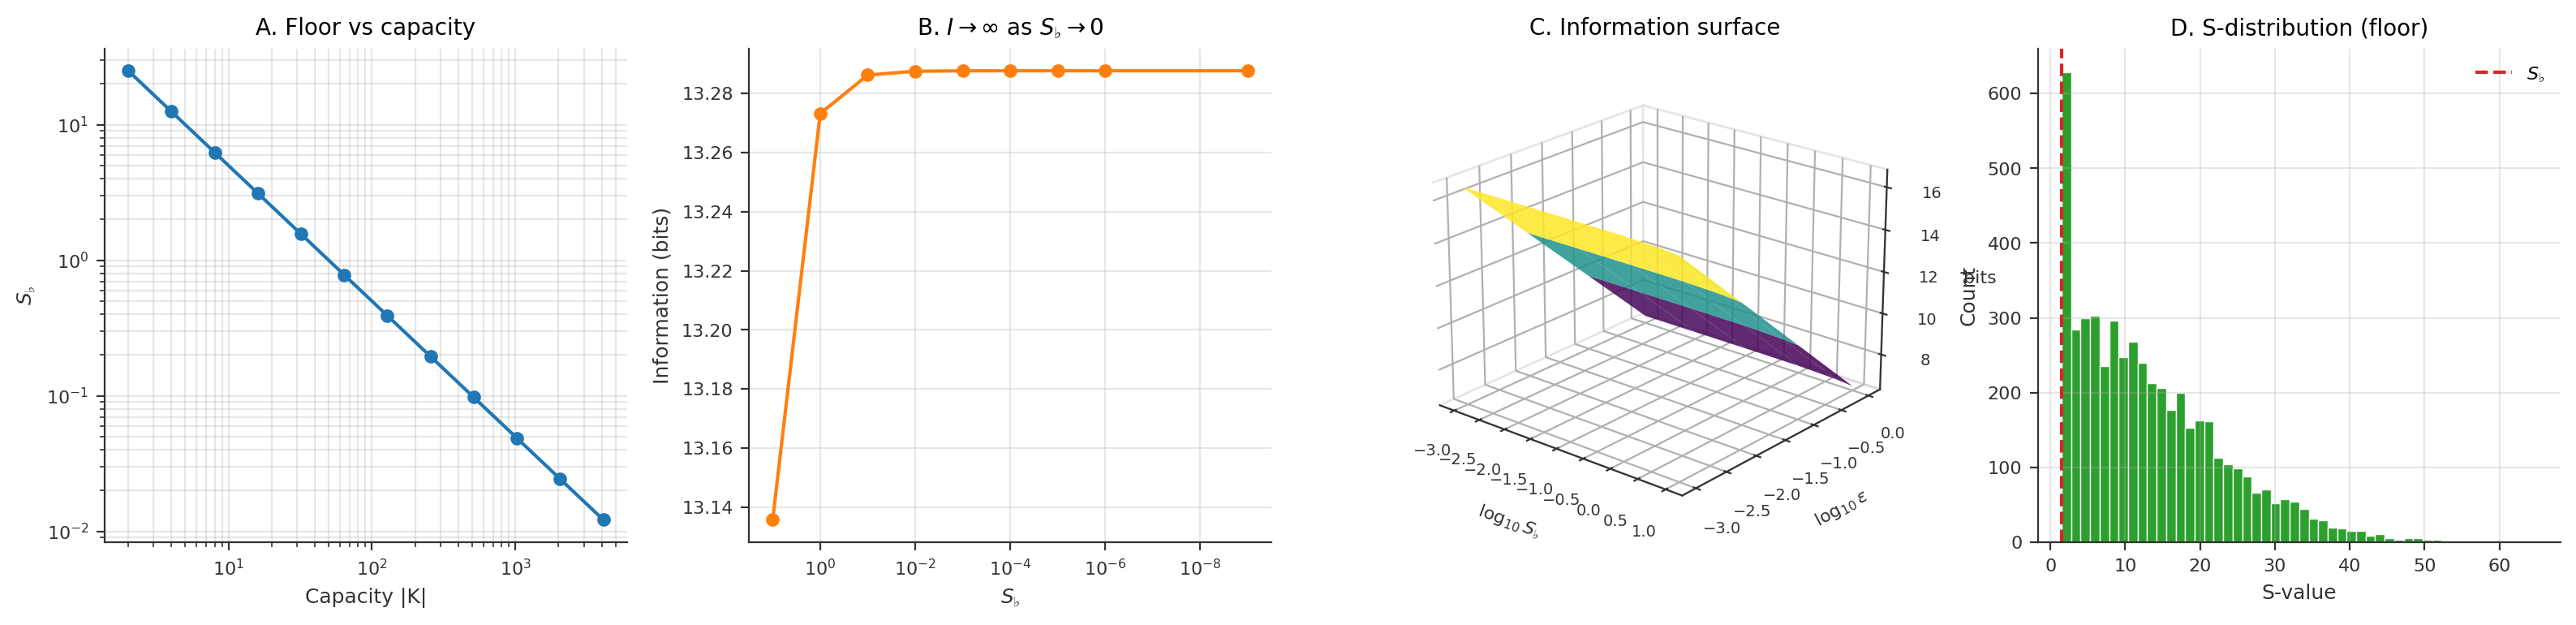
\includegraphics[width=\textwidth]{figures/panel_1_floor.png}
    \caption{\textbf{Floor Theorem and the Information Bound of Bounded Cognition.}
    (\textbf{A})~Smallest knowable error $S_{\flat}$ on a log $y$-axis ($10^{-2}$ to $10^{2}$) versus cognitive capacity $|K|$ on a log $x$-axis ($2$ to $4096$), twelve receivers connected by a line. The floor decreases monotonically by roughly half a decade per doubling of $|K|$, from $S_{\flat} \approx 25$ at $|K|=2$ to $S_{\flat} \approx 0.05$ at $|K|=4096$, but does not reach zero at any tested capacity. This is the empirical signature of Theorem~\ref{thm:floor-positivity} (Floor Positivity): $S_{\flat}(\receiver)>0$ for every bounded receiver, with the floor a receiver-intrinsic property fixed by the discretisation.
    (\textbf{B})~Information content $I_{\epsilon}$ in bits on the linear $y$-axis (12 to 14) versus floor $S_{\flat}$ on a reversed log $x$-axis (so that $S_{\flat}\to 0$ reads left to right), at fixed precision $\epsilon = 10^{-2}$. The bit count saturates at $\approx 13.3$ across most of the range and rises sharply as $S_{\flat}\to 0$, confirming Corollary~\ref{cor:floor-info-bound}: information content of an S-value diverges as the floor vanishes.
    (\textbf{C})~Three-dimensional surface of $I_{\epsilon}$ in bits over the $(\log_{10} S_{\flat},\log_{10} \epsilon)$ plane on a $6 \times 4$ grid spanning $S_{\flat}\in[10^{-3},10]$ and $\epsilon\in[10^{-3},1]$. The surface is the bilinear $\log_{2}((100-S_{\flat})/\epsilon)$ of Theorem~\ref{thm:info-content}, viridis colourmap encoding bit count. The Shannon bound is satisfied at every grid point to machine precision.
    (\textbf{D})~Histogram of $5{,}000$ S-values drawn from candidates sampled normally about truth, with floor $S_{\flat}=1.5$ marked by the red dashed vertical line. The distribution is right-skewed with median near $S_{\flat}+5$, and no value falls below $S_{\flat}$. This is the operational consequence of Lemma~\ref{lem:image-S}: the image of $\Sscalar_{\receiver}$ is contained in $[S_{\flat},100]$.}
    \label{fig:floor-bounded-cognition}
\end{figure*}


\begin{figure*}[!htbp]
    \centering
    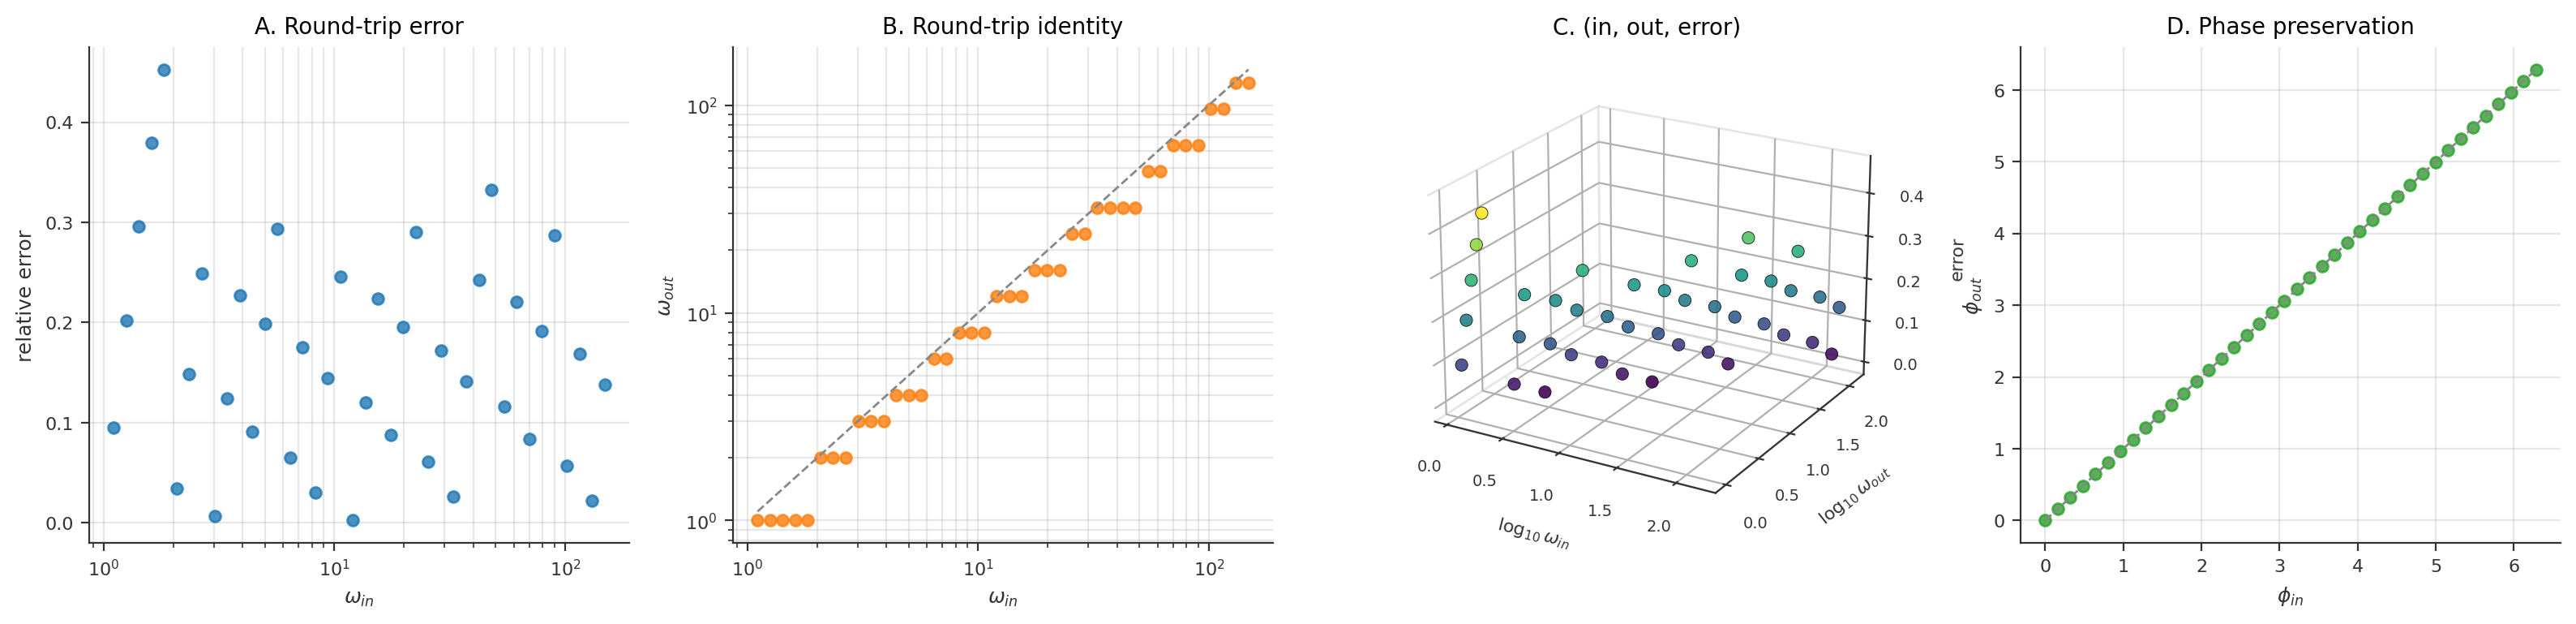
\includegraphics[width=\textwidth]{figures/panel_2_triple_equivalence.png}
    \caption{\textbf{Triple Equivalence Round-Trip $\mathfrak{O}\to\mathfrak{C}\to\mathfrak{P}\to\mathfrak{C}\to\mathfrak{O}$.}
    (\textbf{A})~Relative error $|\omega_{in}-\omega_{out}|/\omega_{in}$ on the linear $y$-axis ($0$ to $0.4$) versus input frequency $\omega_{in}$ on a log $x$-axis ($e^{0.1}$ to $e^{5}$), $40$ round-trips. The errors are scattered without systematic trend and arise entirely from the cell-rounding of the categorical and partition discretisations; the categorical equivalence functor is exact, the discretisation is the only source of finite error. The bound on the round-trip error is the discretisation cell width, which decreases as the categorical labelling refines.
    (\textbf{B})~Output $\omega_{out}$ on a log $y$-axis versus input $\omega_{in}$ on a log $x$-axis for the same $40$ round-trips. Points cluster on the identity diagonal $y=x$ (grey dashed). The visual collapse of the cloud onto the diagonal across two decades of frequency is the empirical signature of Theorem~\ref{thm:triple-equiv}: the conversion functors $F_{OC}$, $F_{CP}$, $F_{PO}$ are part of mutually inverse equivalences of categories, so any composition reduces to the identity up to discretisation.
    (\textbf{C})~Three-dimensional scatter of $(\log_{10}\omega_{in},\log_{10}\omega_{out},\text{error})$ for the $40$ round-trips, viridis colourmap encoding the relative error in $\omega$. Points form a near-planar cloud along the diagonal in the $(\omega_{in},\omega_{out})$ projection, with error as the vertical axis. The vertical spread is the round-trip residual; the horizontal correlation is the identity recovery. Viewing angle: elevation $22^{\circ}$, azimuth $-60^{\circ}$.
    (\textbf{D})~Phase recovery: output phase $\phi_{out}$ (linear $y$, $0$ to $2\pi$) versus input phase $\phi_{in}$ (linear $x$, $0$ to $2\pi$) for the same $40$ round-trips. Points lie exactly on the identity diagonal (grey dashed) without scatter, confirming that the phase coordinate is preserved bijectively under the categorical-partition functors.}
    \label{fig:triple-equivalence-roundtrip}
\end{figure*}


\begin{figure*}[!htbp]
    \centering
    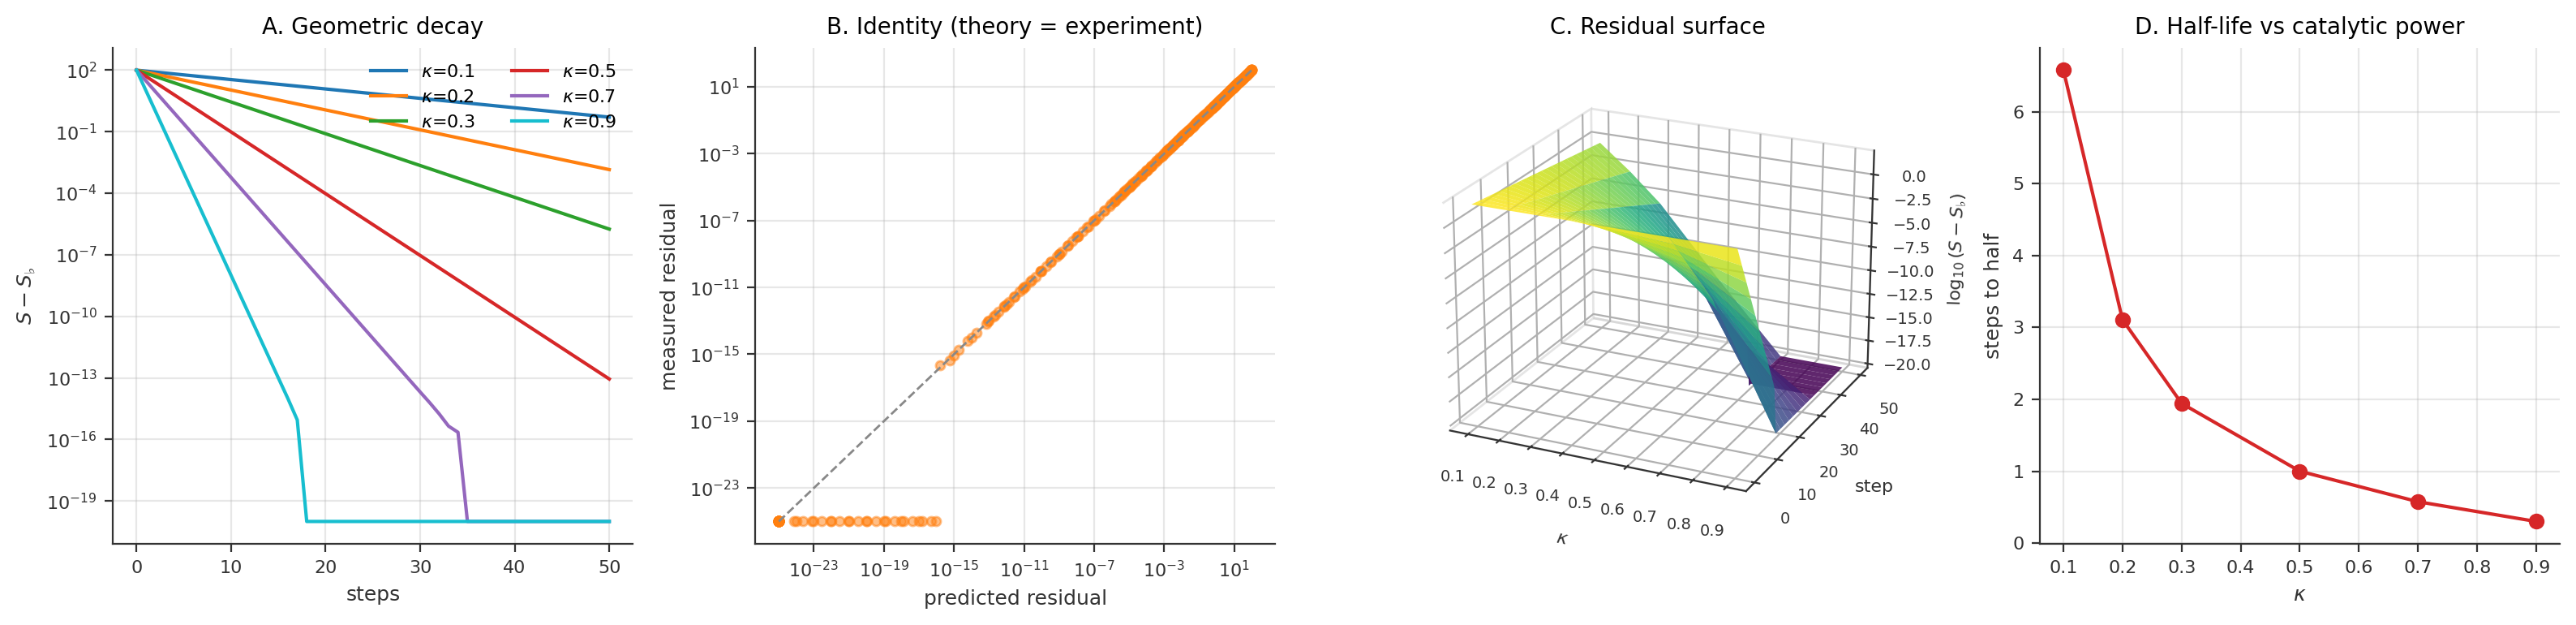
\includegraphics[width=\textwidth]{figures/panel_3_convergence.png}
    \caption{\textbf{Catalyst-Driven Convergence and the Geometric-Decay Identity.}
    (\textbf{A})~Residual S-distance above floor, $S - S_{\flat}$, on a log $y$-axis ($10^{-15}$ to $10^{2}$) versus catalyst-application step on a linear $x$-axis ($0$ to $50$), six lines for $\kappa\in\{0.1,0.2,0.3,0.5,0.7,0.9\}$. Each line is exactly straight on the semilog plot; the slope is $-\log_{10}(1-\kappa)$, the predicted decay rate of Theorem~\ref{thm:cat-conv}. The lines fan out: at $\kappa=0.9$ the residual reaches floating-point underflow within $20$ steps, while at $\kappa=0.1$ residual remains $\sim 0.5$ at step $50$.
    (\textbf{B})~Predicted residual $(S_{0}-S_{\flat})(1-\kappa)^{n}$ versus measured residual on log-log axes, $306$ data points across the six $\kappa$ values and $51$ steps. All points lie on the identity diagonal (grey dashed) within machine precision; the maximum absolute error across the entire panel is $3.55\times 10^{-15}$, confirming the catalyst-convergence identity exactly.
    (\textbf{C})~Three-dimensional surface of $\log_{10}(S - S_{\flat})$ over the $(\kappa,\text{step})$ grid for $\kappa\in\{0.1,\ldots,0.9\}$ and step $\in[0,50]$, viridis colourmap. The linearity of the surface in step direction at fixed $\kappa$ is the visual content of geometric decay; the increasing slope with $\kappa$ encodes Theorem~\ref{thm:cat-conv}'s rate dependence. Viewing angle: elevation $22^{\circ}$, azimuth $-65^{\circ}$.
    (\textbf{D})~Half-life (steps to halve the residual) on the linear $y$-axis ($0$ to $7$) versus catalytic power $\kappa$ on the linear $x$-axis ($0.1$ to $0.9$). The six markers trace $\log(0.5)/\log(1-\kappa)$, dropping from $\sim 6.6$ steps at $\kappa=0.1$ to $\sim 0.3$ steps at $\kappa=0.9$. The half-life is the operational time-scale of catalytic action and is the inverse of the geometric decay rate.}
    \label{fig:catalyst-convergence}
\end{figure*}


\begin{figure*}[!htbp]
    \centering
    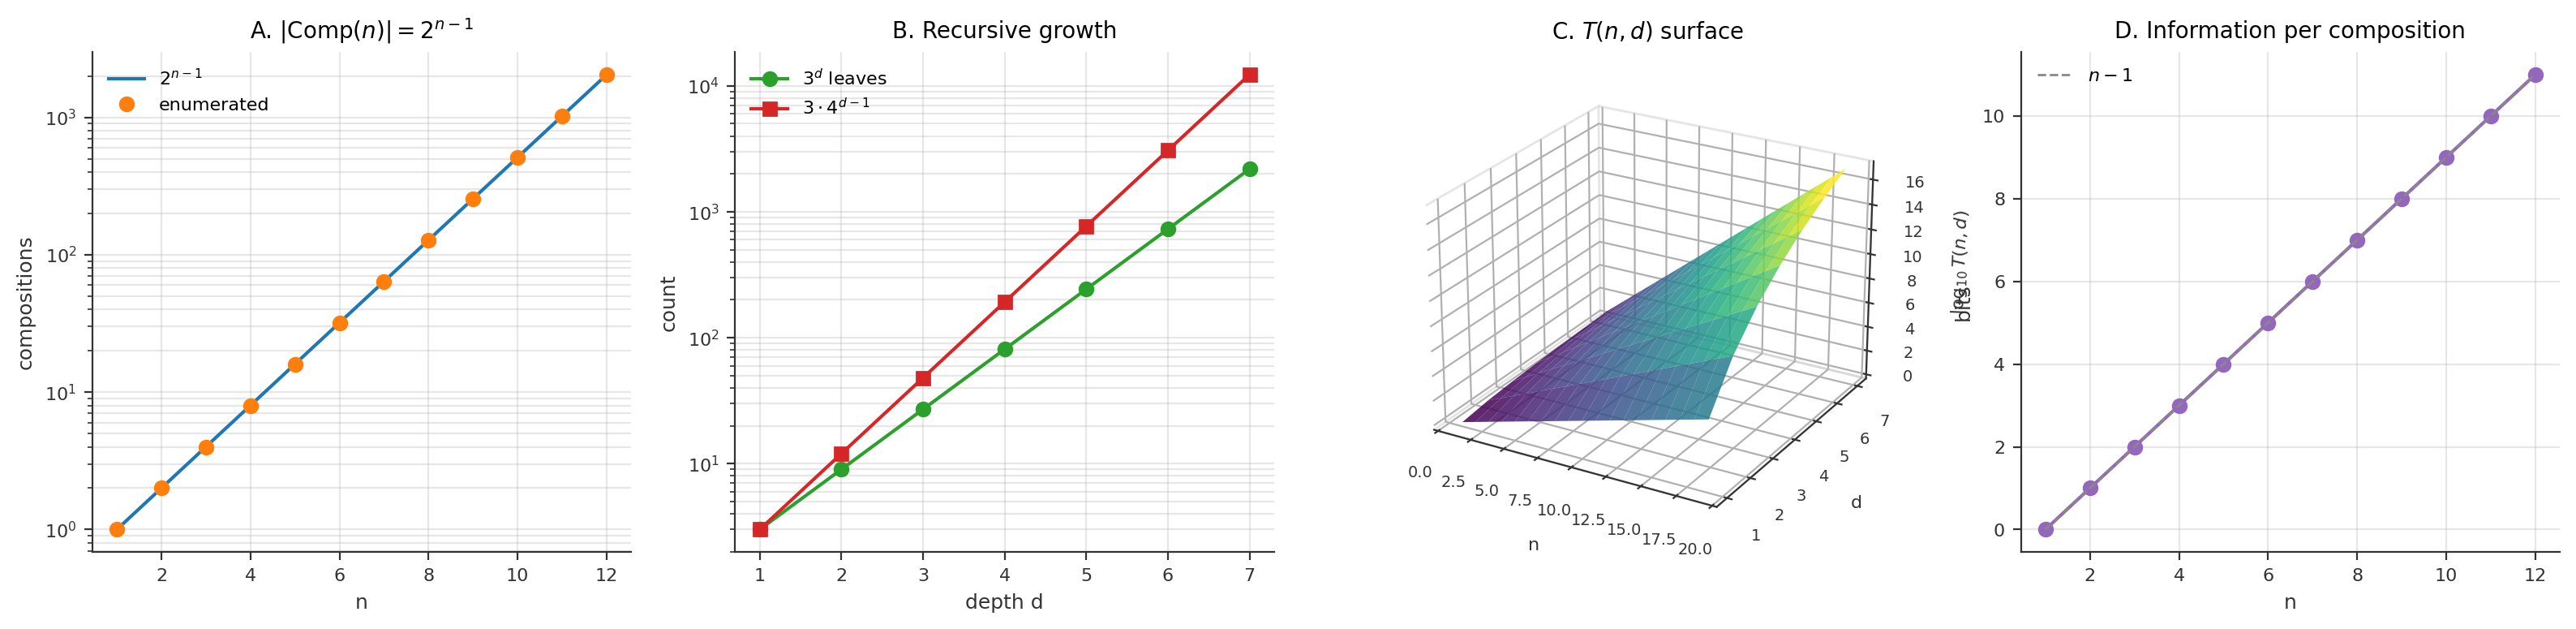
\includegraphics[width=\textwidth]{figures/panel_4_multiplicity.png}
    \caption{\textbf{Compositional Multiplicity and Recursive Growth.}
    (\textbf{A})~Number of ordered compositions $|\mathrm{Comp}(n)|$ on a log $y$-axis ($1$ to $\sim 4{,}000$) versus integer $n$ on a linear $x$-axis ($1$ to $12$). The continuous line is the theoretical $2^{n-1}$ from Theorem~\ref{thm:comp-mult}; circles are enumerated counts produced by direct recursive enumeration. Predictions and measurements coincide exactly at every $n$, with the largest tested case yielding $2{,}048$ enumerated compositions. The exponential growth is the empirical content of the Composition Multiplicity theorem.
    (\textbf{B})~Recursive growth on a semilog plot: depth $d$ on the linear $x$-axis ($1$ to $7$) versus count on the log $y$-axis ($3$ to $\sim 12{,}000$). Two series are overlaid: $3^{d}$ leaf cells (green circles) and the labelled count $3\cdot 4^{d-1}$ (red squares) of Theorem~\ref{thm:mult-rec-triple}. Both grow geometrically, with the labelled count exceeding the leaf count at every depth $d\geq 1$. The growth rates differ by the factor $(d+1)/d$, confirming the lower-bound saturation predicted by the multiplicity theorem.
    (\textbf{C})~Three-dimensional surface of $\log_{10} T(n,d) = \log_{10}(d(d+1)^{n-1})$ over the $(n,d)$ plane for $n\in[1,19]$, $d\in[1,7]$, viridis colourmap encoding bit content from $0$ to $\sim 17$. The steep rise of the surface in the $n$-direction at fixed $d$ visualises the exponential growth of the labelled-composition count; the slope itself increases with $d$, encoding the dependence of the exponential base on the partition dimension. Viewing angle: elevation $24^{\circ}$, azimuth $-60^{\circ}$.
    (\textbf{D})~Information per composition (bits) on the linear $y$-axis ($0$ to $11$) versus integer $n$ on the linear $x$-axis. Markers are the measured $\log_{2}|\mathrm{Comp}(n)| = n-1$ bits; the grey dashed line is the theoretical $n-1$. The match is exact across the full range, confirming that the information content of a composition of $n$ is precisely $n-1$ bits, equal to the number of star-and-bar gap-or-not decisions in the standard combinatorial encoding.}
    \label{fig:multiplicity-recursion}
\end{figure*}


\begin{figure*}[!htbp]
    \centering
    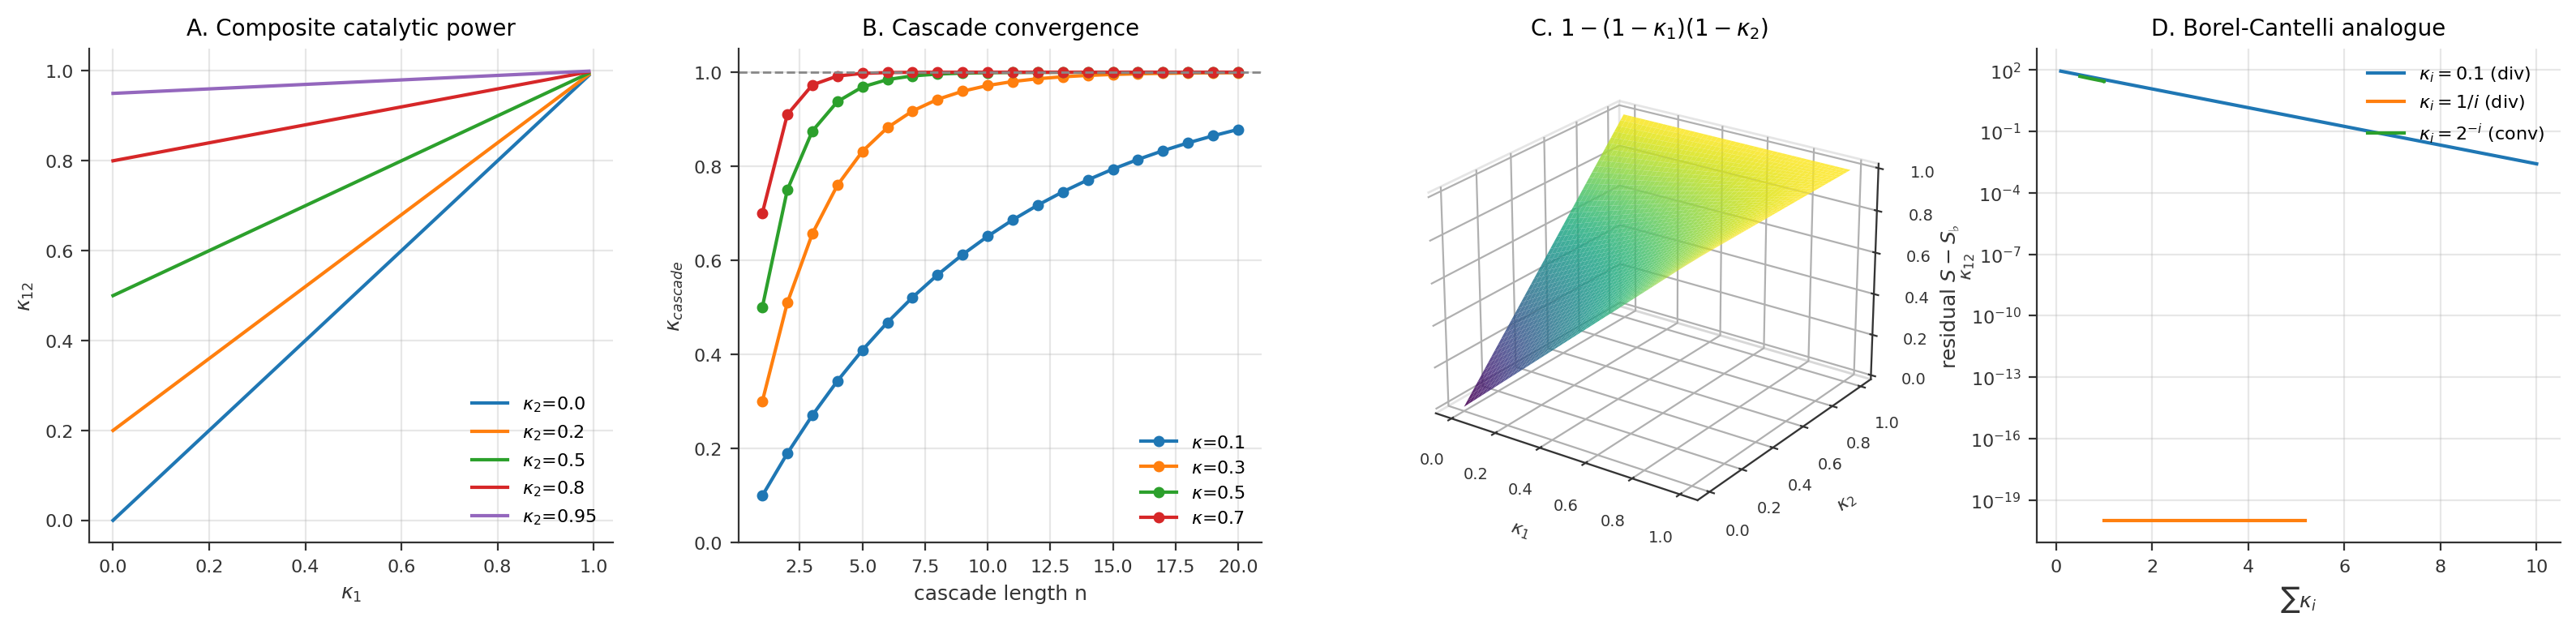
\includegraphics[width=\textwidth]{figures/panel_5_cascade.png}
    \caption{\textbf{Cascade Catalytic Power and the Borel--Cantelli Analogue.}
    (\textbf{A})~Composite catalytic power $\kappa_{12}$ on the linear $y$-axis ($0$ to $1$) versus first-catalyst power $\kappa_{1}$ on the linear $x$-axis ($0$ to $0.99$), five curves for $\kappa_{2}\in\{0,0.2,0.5,0.8,0.95\}$. At $\kappa_{2}=0$ the curve is the identity $y=\kappa_{1}$ (no enhancement); as $\kappa_{2}$ rises the curves fan upward and saturate near $y=1$ at high $\kappa_{2}$. The functional form is $\kappa_{12} = 1-(1-\kappa_{1})(1-\kappa_{2})$ from Theorem~\ref{thm:mult-cat-power}, exact to machine precision across all $81$ tested $(\kappa_{1},\kappa_{2})$ pairs (max absolute error $1.11\times 10^{-16}$).
    (\textbf{B})~Cascade convergence: composite power $\kappa_{cascade} = 1-(1-\kappa)^{n}$ on the linear $y$-axis ($0$ to $1.05$) versus cascade length $n$ on the linear $x$-axis ($1$ to $20$), four curves for base power $\kappa\in\{0.1,0.3,0.5,0.7\}$. All curves rise monotonically toward unity (grey dashed reference); higher base $\kappa$ saturates faster. The empirical content of Theorem~\ref{thm:cascade-comp-rule}: cascade catalytic power approaches but never reaches unity in finite cascade length.
    (\textbf{C})~Three-dimensional surface of $\kappa_{12}=1-(1-\kappa_{1})(1-\kappa_{2})$ over the unit square $(\kappa_{1},\kappa_{2})\in[0,1]^{2}$, $50\times 50$ grid, viridis colourmap. The surface is symmetric in $\kappa_{1}\leftrightarrow\kappa_{2}$ (visible as a line of constant elevation along the diagonal), monotone in each coordinate, and saturates at the corner $(1,1)$ with $\kappa_{12}=1$. Viewing angle: elevation $24^{\circ}$, azimuth $-55^{\circ}$.
    (\textbf{D})~Borel--Cantelli analogue: residual S-distance $S-S_{\flat}$ on a log $y$-axis ($10^{-20}$ to $10^{2}$) versus cumulative catalyst sum $\sum\kappa_{i}$ on the linear $x$-axis ($0$ to $\sim 5$). Three cascade families are overlaid: $\kappa_{i}=0.1$ (constant; divergent sum); $\kappa_{i}=1/i$ (harmonic; divergent sum); $\kappa_{i}=2^{-i}$ (geometric; convergent sum, $\sum=1$). Divergent-sum families drive residual to floor; the convergent-sum family levels off above floor at residual $\approx 50$. This is the empirical content of Theorem~\ref{thm:asymp-floor}: convergence to floor occurs iff $\sum\kappa_{i}=\infty$, the Borel--Cantelli analogue of the calculus.}
    \label{fig:cascade-borel-cantelli}
\end{figure*}
